\subsubsection{Evaluation verfügbarer Produkte}
\label{chap:produkt-eval}
\paragraph{Auswahl der \ac{WAF}-Anwendung}

\paragraph{Verwundbare Anwendungen}

\subsubsection{Labor-Umgebung}

% 1. Anforderungen an die Lernumgebung
% 2. Überlegungen zur gestaltung einheiltichen Deployments
% 2.1. Docker
%       - einheitlich
%       - Netzwerke
%       - Probleme mit croscompatibility (Windows)
% 2.2. VM (vortiele und Probleme)
% 3. beschreibung der Container
% 3.1. Juicesop
% 3.2. WAF
% 3.3. Python contaienr mit test script

Die in Kapitel \ref{chap:inhalte} beschriebenen Inhalte sollen in einem Praxisnahen Umfeld vermittelt werden.
Dazu kommt nach den Abwägungen aus Kapitel \ref{chap:produkt-eval}, die Waf-Applikation ModSecurity zum Einsatz.
Die zu diesem Zweck vorgesehene Laborumgebung muss einige Kriterien erfüllen:
\begin{description}
    \item[Einheitliches Deployment:] Der Ausgangspunkt der Lerneinheiten muss reproduzierbar und wiederholbar sein. Bei wiederholten Durchführungen der Übungen soll es einfach sein den Lernenden ohne zusätzlichem manuellen Konfigurationsaufwand eine Laborumgebung zu übergeben. Diese Laborumgebung muss Platform-unabhängig aufgebaut sein und auf Windows, MacOS unf Linux genutzt werden können.
    \item[Modifizierbarketit der Anwendungen:] Um in den Lerneinheiten grundlegende Techniken zu übermitteln, ist es notwendig Basis-Funktion der ModSecurity \ac{waf} entfernen zu können. Dies muss automatisierten und einheitlichen Weg erfolgen können.
    \item[Bekannte Basis-Technologien:] Der Fokus der Lerneinheiten liegt auf dem Erlernen der Technik und Funktion einer \ac{waf}. Um einen Einstieg möglichst direkt zu gestalten sollen hierfür Technologien zuj Einsatz kommen, die den Lernenden schon bekannt sind und keinen zusätzlichen Lernaufwand erzeugen.
    \item[Komplexe Netzwerkumgebungen:] Da die verschiedenen Anwendungen in der Laborumgebung über Netzwerkkommunikation miteinander sprechen, muss es möglich sein automatisiert virtuelle Netzwerke zu erzeugen.
\end{description}

Um den oben genannten Anforderungen möglichst genau zu entsprechen, wurde die in Abbildung \ref{fig:lab} schematisch dargestellte Umgebung erstellt.

\begin{figure}[!hbt]
    \centering
    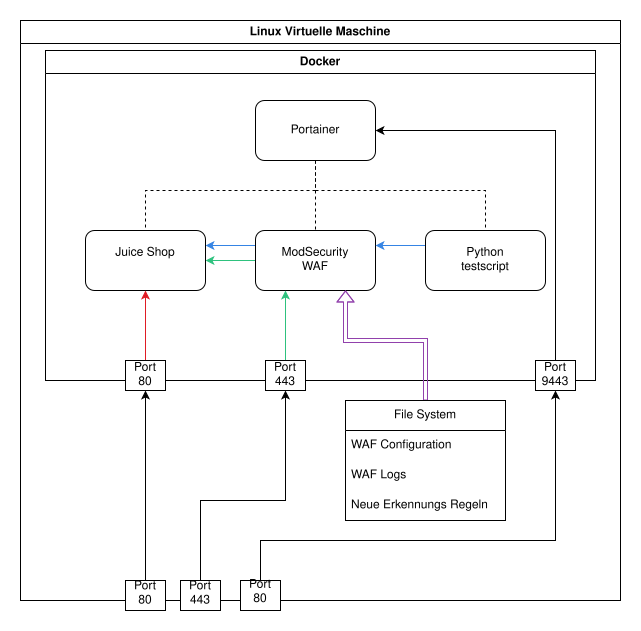
\includegraphics[width=0.9\textwidth]{./images/lab-setup.png}
    \caption{Aufbau der Laborumgebung}
    \label{fig:lab}
\end{figure}

Als basis deployment Technologie wird die Containervirtualisierungsumgebung Docker verwendet. Die ermöglicht es 